\subsection{Анализ исполнений}

На картинке приведен пример исходного Roren графа (рис.~\ref{fig:roren1}) и полученный из него граф операций YT (рис.~\ref{fig:ytgraph}).

\begin{figure}[h]
    \centering
    \includegraphics[width=\textwidth]{img/roren1.png}
    \caption{Неоптимизированный roren граф из ParDo}
    \label{fig:roren1}
\end{figure}

\begin{figure}[h]
    \centering
    \includegraphics[width=\textwidth]{img/ytgraph.png}
    \caption{Итоговый YT граф}
    \label{fig:ytgraph}
\end{figure}

Также есть возможность изучить Roren графы полученные на промежуточных этапах: после удаления Flatten (рис.~\ref{fig:roren2}), после оптимизации (рис.~\ref{fig:roren3}) и подграф сконденсированный в единственную вершину (рис.~\ref{fig:subgraph})

\begin{figure}[h]
    \centering
    \includegraphics[width=\textwidth]{img/roren2.png}
    \caption{Roren граф из ParDo после предобхода Flatten}
    \label{fig:roren2}
\end{figure}

\begin{figure}[h]
    \centering
    \includegraphics[width=\textwidth]{img/roren3.png}
    \caption{Roren граф из ParDo после основного обхода}
    \label{fig:roren3}
\end{figure}

\begin{figure}[h]
    \centering
    \includegraphics[width=\textwidth]{img/subgraph.png}
    \caption{Подграф полностью оптимизированного roren графа}
    \label{fig:subgraph}
\end{figure}

Также приведем пример для roren графа (рис.~\ref{fig:mrroren}), который результирует в единственную операцию MapReduce (рис.~\ref{fig:mrytgraph}).

\begin{figure}[h]
    \centering
    \includegraphics[width=\textwidth]{img/mrroren.png}
    \caption{Roren граф из ParDo и GroupByKey (цифра 2 на рисунке) до оптимизаций}
    \label{fig:mrroren}
\end{figure}

\begin{figure}[h]
    \centering
    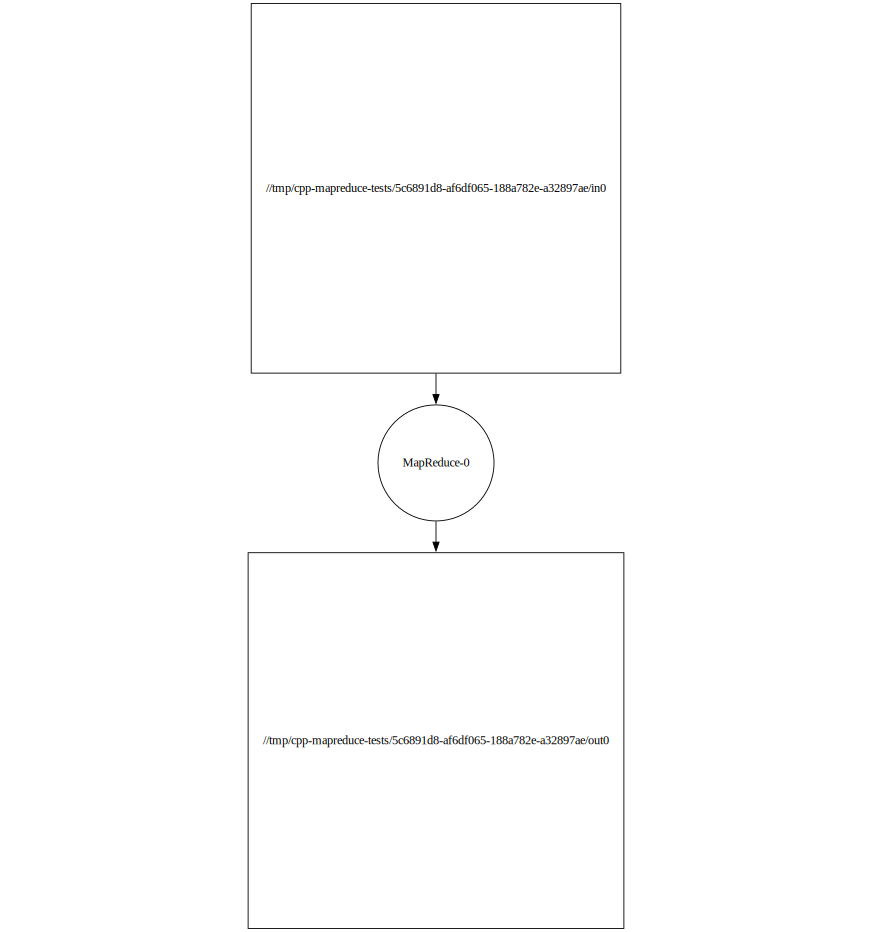
\includegraphics[width=\textwidth]{img/mrytgraph.png}
    \caption{Итоговый YT граф с одной MapReduce операцией}
    \label{fig:mrytgraph}
\end{figure}

Ниже прикреплены скриншоты соответствующие Map (рис.~\ref{fig:ytop}) и MapReduce (рис.~\ref{fig:mrytop}) job-ам из двух предыдущих примеров.

\begin{figure}[h]
    \centering
    \includegraphics[width=\textwidth]{img/ytop.png}
    \caption{Спецификация Map операции запущенной на кластере YT}
    \label{fig:ytop}
\end{figure}

\begin{figure}[h]
    \centering
    \includegraphics[width=\textwidth]{img/mrytop.png}
    \caption{Спецификация MapReduce операции запущенной на кластере YT}
    \label{fig:mrytop}
\end{figure}
